\documentclass{article}
\usepackage{amsmath}
\usepackage{amsfonts} 
\usepackage{graphicx}
\usepackage{biblatex} 
\usepackage{authblk}
\usepackage{mathtools}
\usepackage{xurl} %see https://tex.stackexchange.com/questions/23394/url-linebreak-in-footnote for why we use xurl to get line breaks instead of regular url
\usepackage{hyperref}
\usepackage{listings}
\usepackage{cancel}
\usepackage{enumitem}
\usepackage[bb=boondox]{mathalfa}
\addbibresource{three_books.bib}
\DeclareMathOperator*{\argmax}{arg\,max}
\DeclareMathOperator*{\argmin}{arg\,min}

\setlist[description]{leftmargin=2cm,labelindent=1cm}

\lstdefinestyle{mystyle}{
    % backgroundcolor=\color{backcolour},   
    % commentstyle=\color{codegreen},
    % keywordstyle=\color{magenta},
    % numberstyle=\tiny\color{codegray},
    % stringstyle=\color{codepurple},
    % basicstyle=\ttfamily\footnotesize,
    % breakatwhitespace=false,         
    % breaklines=true,                 
    captionpos=b,                    
    keepspaces=true,                 
    % numbers=left,                    
    % numbersep=5pt,                  
    % showspaces=false,                
    % showstringspaces=false,
    % showtabs=false,                  
    tabsize=2,
    frame=single,
}
\lstset{style=mystyle}

\title{Blueprints for building reinforcement learning algorithms in customer-facing applications}
\author[1]{Douglas Mason}
\affil[1]{Koyote Science, LLC \footnote{\href{http://www.koyotescience.com}{\texttt{http://www.koyotescience.com}}}}
\date{November 2021}

\begin{document}

\maketitle

\section{Introduction}
This document outlines primary considerations for designing production-worthy reinforcement learning algorithms in customer-facing settings. We will (1) establish the notation, (2) discuss how policies are evaluated, (3) show how policies can be defined by evaluation functions alone, (4) demonstrate how we train an evaluation for our policy, even from customer interactions driven by another policy, known as off-policy training, (5) show how we can train the policy directly from customer interactions, and (6) demonstrate how we can combine both approaches for the current state-of-the-art in the field. We also (7) provide practical considerations under the hood for building our policies and evaluation functions, as well as (8) additional resources to help the reader dive more deeply into the field, as well as discover implementations that can be used right now. This document attempts to be brief but mathematically thorough. Please write to the author at \href{mailto:douglas@koyotescience.com}{douglas@koyotescience.com} for questions or feedback. We provide a quick schematic of the algorithms we will cover in Figure \ref{fig:rl_schematic}.
\begin{figure}\label{fig:rl_schematic}
    \begin{center}
    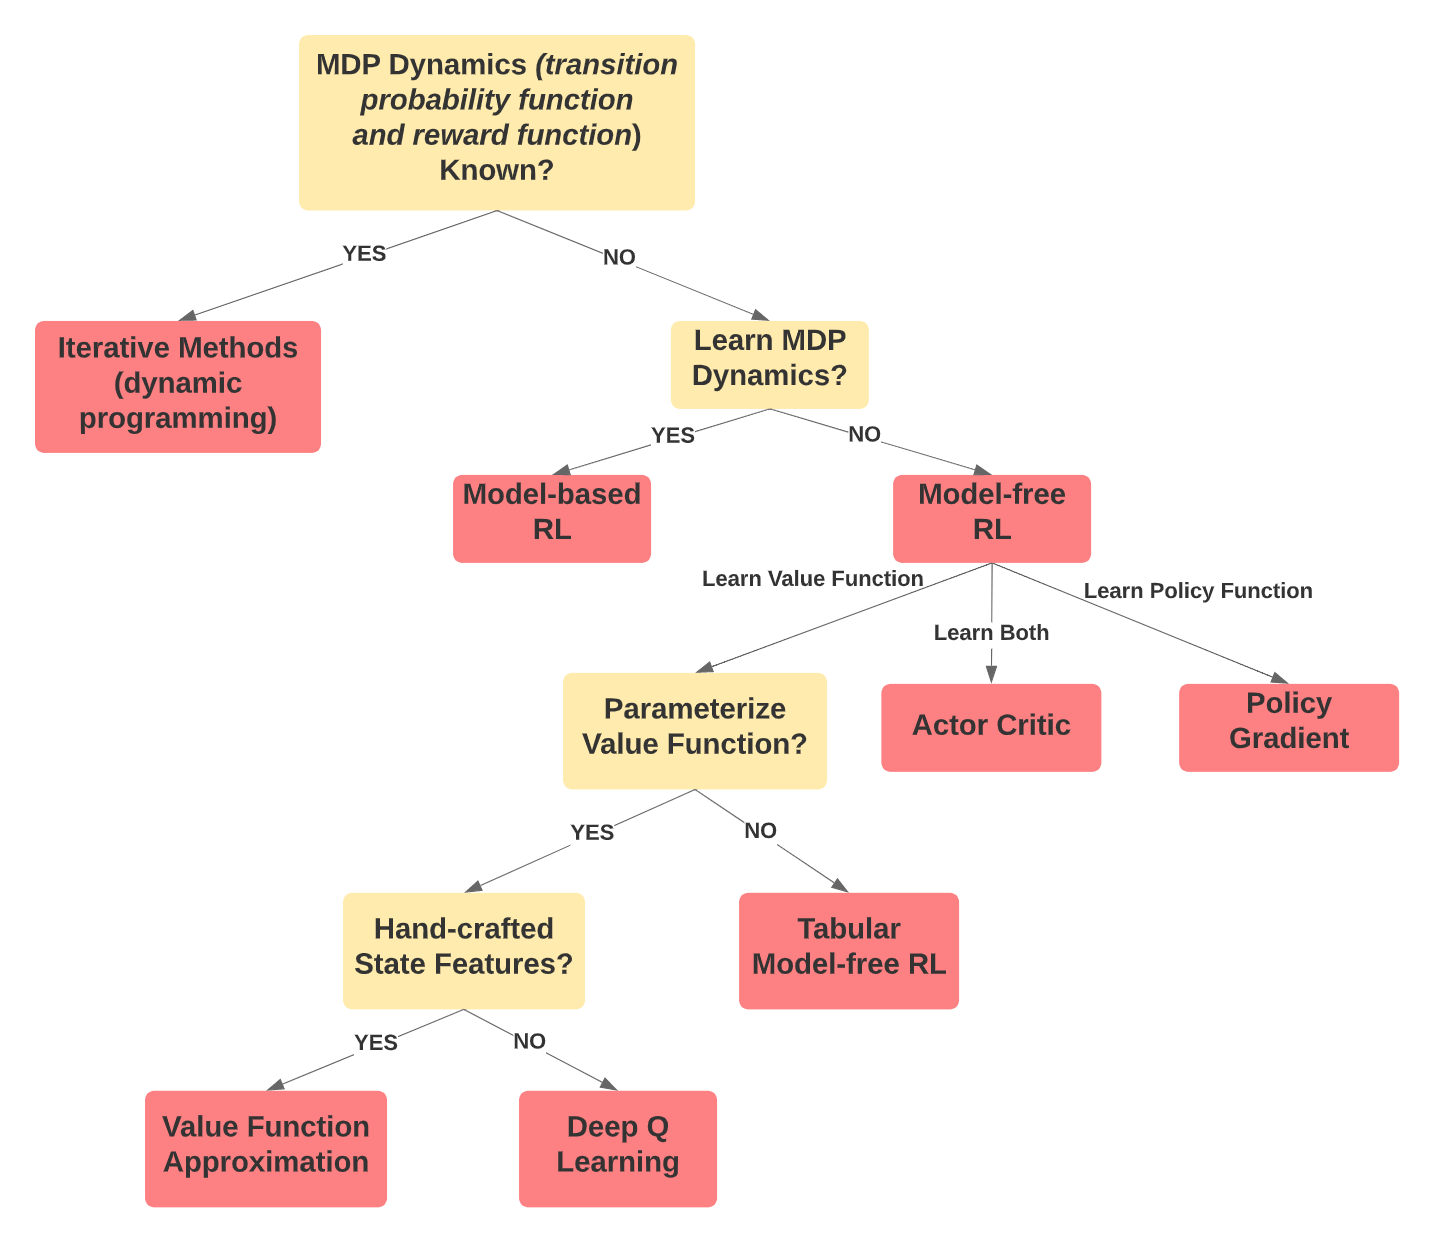
\includegraphics[width=0.75\linewidth]{rl_schematic}
    \caption{Schematic for the reinforcement learning approaches covered in this document.\footnotemark}
    \end{center}
\end{figure}
\footnotetext{ Source: \url{https://towardsdatascience.com/an-overview-of-classic-reinforcement-learning-algorithms-part-1-f79c8b87e5af}}

At a high-level overview, reinforcement learning algorithms consist of up to three primary components:
\begin{enumerate}
\item A \textit{policy evaluator}, which can be used to define the policy on its own. This is often referred to as the state- or action-value function.
\item A \textit{policy function}, which defines the policy on its own, and can use a policy evaluator to improve its performance
\item A \textit{rollout planning} system for using the policy evaluator and policy function to fine-tune performance
\end{enumerate}
This documents covers the first two components, and lightly touches on the third, since it is the riskiest to implement in a production system, and requires the ability to predict future states of the system, known as the \textit{environment model}. Moreover, the policy evaluator is a development of the multi-armed bandit formalism, allowing it to act as a stepping stone between optimization, such as hyperparameter tuning, and sequential planning that uses an explicit policy function.

\section{Notation and policy evaluation}

When designing products that take users through a sequence of actions to get to a desired goal, it’s a natural instinct to look at the field of reinforcement learning to optimize your design. In this formulation, we have a state vector $\mathbf{s}$ (e.g., the current page a user is on) which may also incorporate a context vector $\mathbf{c}$ (e.g., user demographics), an action vector $\mathbf{a}$ that represents a decision that the system can take (e.g., presenting different options along the way), and a reward for taking an action at a given state $r(\mathbf{s},\mathbf{a})$ (e.g., whether a user signs up at the end of a sign-up flow). Note that we can also define the reward without considering the action, $r(\mathbf{s})$, which is identical except that it is defined by the state you end up in to get the reward rather than the state and action you take to get it. 

We are interested in learning a policy $\pi(\mathbf{a}| \mathbf{s})\in [0,1]$ that gives us the probability of choosing a given action $\mathbf{a}$ with a given state $\mathbf{s}$. Note that when implemented, such a function depends on both $\mathbf{a}$ and $\mathbf{s}$. The policy is normalized so that its returns for all available actions at a given state add up to one, i.e., \begin{equation}\label{eq:normalization}
\sum_\mathbf{a}\pi(\mathbf{a}|\mathbf{s})=1
\end{equation} When learning this policy, our goal is to maximize the discounted sum of future rewards $G_t(\boldsymbol{\tau})$\footnote{The letter $G$ is chosen for historical reasons, while $J(\pi_{\boldsymbol{\theta}})=\mathop{\mathbb{E}}_{\boldsymbol{\tau}\sim\pi_{\boldsymbol{\theta}}}[G_0({\boldsymbol{\tau}})]$ is used later in Equation \ref{eq:J}} from time step $t$ through the problem horizon $H$, as we step through a given trajectory of states $\boldsymbol{\tau}$ which we write out as
\begin{equation}
\boldsymbol{\tau}=(\mathbf{s}_0,\mathbf{a}_0,\mathbf{s}_1,\mathbf{a}_1,\dots,\mathbf{s}_H,\mathbf{a}_H)
\end{equation} and where the discount factor $\gamma\in(0,1]$. We write this quantity out as
\begin{equation}
    G_t(\boldsymbol{\tau})=\sum_{t'=t}^{H}r(\mathbf{s}_{t'},\mathbf{a}_{t'})\gamma^{t'-t}
\end{equation}
We can accomplish this by learning a Q-value or action-value function for each state and action, which returns the expected discounted sum of future rewards assuming we follow a policy $\pi$ starting from state $\mathbf{s}$ and action $\mathbf{a}$, and can be written as
\begin{equation}
\begin{split}
Q_\pi(\mathbf{s},\mathbf{a})&=\mathop{\mathbb{E}}_{\boldsymbol{\tau}\sim\pi}[G_t({\boldsymbol{\tau}})|\mathbf{s}_t=\mathbf{s},\mathbf{a}_t=\mathbf{a}]\\&=\sum_{t'=t}^{H}\pi(\mathbf{a}_{t'}|\mathbf{s}_{t'})r(\mathbf{s}_{t'},\mathbf{a}_{t'})\gamma^{t'-t}
\end{split}
\end{equation} Other formulations may work with a state-value function \begin{equation}\begin{split}V_{\pi}(\mathbf{s})&=\sum_{\mathbf{a}\sim\mathcal{A}}\pi(\mathbf{a}|\mathbf{s})Q_\pi(\mathbf{s},\mathbf{a})\\&=\mathop{\mathbb{E}}_{\boldsymbol{\tau}\sim\pi}[G_t({\boldsymbol{\tau}})|\mathbf{s}_t=\mathbf{s}]\\&=\sum_{t'=t}^{H}\sum_{\mathbf{a}\sim\mathcal{A}}\pi(\mathbf{a}_{t'}|\mathbf{s}_{t'})r(\mathbf{s}_{t'},\mathbf{a}_{t'})\gamma^{t'-t}\end{split}\end{equation}which only depends on the state.

\section{Deriving the policy from the evaluation}
The policy can be determined by the $Q$-value using a greedy strategy
\begin{equation}\label{eq:greedy_policy}
    \pi(\mathbf{a}|\mathbf{s})=\mathbb{1}\left[\mathbf{a}=\argmax_\mathbf{a}Q(\mathbf{s},\mathbf{a}))\right]
\end{equation}where $\mathbb{1}[\cdot]$ returns a 1 when the argument is true and 0 otherwise. This policy is deterministic, but we can make a stochastic policy using a variety of other strategies. In $\epsilon$-greedy, the greedy action is chosen with a fixed probability (say, 75\%), and other actions are chosen at random for the remaining 25\% of the time. Another strategy is to use the softmax function
\begin{equation}
  \pi(\mathbf{a}|\mathbf{s})=\frac{\exp(Q(\mathbf{s},\mathbf{a}))}{\sum_\mathbf{a}\exp(Q(\mathbf{s},\mathbf{a})}
\end{equation}And yet another strategy is to perform gradient ascent against the $Q$-value (when such gradients are available) to maximize it over the action space, which is used in the "deterministic policy gradient" algorithm\cite{DDPG}. If we use the state-value instead of the action-value, then we need to know how actions lead to state transitions, which is outside the scope of this article, and falls under the domain of "model-based" reinforcement learning \cite{model_based_rl_survey}. Note that the word "model" here refers to a model of the environment ($p(\mathbf{s}_{t+1}|\mathbf{s},\mathbf{a}$) as opposed to the models that are used for the policy function or state- and action-value function approximation.

If we define the policy entirely by the state-value function, then we obtain \begin{equation}\pi(\mathbf{a}|\mathbf{s})=\mathbb{1}\left[\mathbf{a}=\argmax_{\mathbf{a}_t}\left(r(\mathbf{s}_t,\mathbf{a}_t)+p(\mathbf{s}_{t+1}|\mathbf{s}_t,\mathbf{a}_t)V(\mathbf{s}')\right)\right]\end{equation}which requires us to also learn an environment model in the form of $p(\mathbf{s}'|\mathbf{s},\mathbf{a})$. While training the state-value function is analogous to training the action-value function, defining a policy based on it is not due to the lack of action dependence. While we do not cover model-based reinforcement learning in this document, we lightly touch on how it can be learned here for the reader's curiosity, and to introduct the concept of importance sampling. 

Given transitions observed by the environment, $p_\text{obs.}(\mathbf{s}'|\mathbf{s},\mathbf{a})$ which sum to one over all possible states $\mathbf{s}'$, we can sample transitions using any policy $\pi$ by storing or learning a function approximator to \begin{equation}p(\mathbf{s}'|\mathbf{s},\mathbf{a})=\mathop{\mathbb{E}}_{\boldsymbol{\tau}\sim\pi}\left[\rho(\mathbf{a}_t|\mathbf{s}_t)p_\text{obs.}(\mathbf{s}_{t+1}|\mathbf{s_t},\mathbf{a}_t)\mathbb{1}\left[\mathbf{s}_t=\mathbf{s},\mathbf{a}_t=\mathbf{a},\mathbf{s}_{t+1}=\mathbf{s}'\right]\right]\end{equation}where the \textit{importance sampling ratio}
\begin{equation}\rho(\mathbf{a}|\mathbf{s})=\frac{\pi_\text{random}(\mathbf{a}|\mathbf{s})}{\pi(\mathbf{a}|\mathbf{s})}\end{equation}is the relative likelihood of choosing that action randomly according to policy $\pi_\text{random}$ compared to the likelihood of choosing it with the policy used to sample trajectories $\pi$. When used in this context, the quantity is sometimes called the \textit{inverse propensity weight} or \textit{inverse propensity score} since it is defined as the inverse of the propensity of that transition under policy $\pi$, where "propensity" is used as a rarer synonym for "probability" to help distinguish it from other probabilities that are also often labeled with the Greek letter $\rho$.

Another strategy makes use of Bayesian models that possess the ability to sample their parameters according to their epistemic uncertainty \cite{GP_BLR}, and is called Thompson sampling \cite{thompson_sampling}. In this strategy, the model parameters are sampled, the $Q$-value is calculated from this sampled model for each available action, and the strategy chooses the action with the highest score. This approach has been shown to optimize the exploration-exploitation trade-off in bandits\cite{thompson_sampling,bootstrap_DQN}. The use of Bootstrap Thompson Sampling (BTS), which approximates the Bayesian distribution by training an ensemble of non-Bayesian models on different bootstrap samples of the training data, was popularized by the algorithm group at Facebook for its engineering benefits, among them that prediction only requires one non-Bayesian model from the ensemble at a time, and debugging is straightforward\cite{bootstrap_facebook}. Further developments, such as Randomized Least Squares Value Iteration, use epistemic uncertainty sampling even when determining the next-state maximizing action in the $Q$-learning phase\cite{RLSVI} to encourage exploration.

Lastly, a recent and amazingly-successful strategy, called Monte Carlo Tree Search (MCTS), performs simulations during each planning stage, using a simplified policy and an environment model, where the simplified policy is guided by state- and/or value-functions that are also trained. These strategies have been very successful in perfect-information, adversarial games, but they are outside the scope of this overview. Read Section 8.11 of \cite{sutton_barto_rl} as well as \cite{go1} and \cite{go2} to learn more.

\section{Training the state- and value-function policy evaluators\label{sec:value_training}}

With this notation secured, we can finally bring in the \textbf{Bellman equation}, which is a major foundation of both reinforcement learning and dynamic programming. It states that the best choices we make now can be determined greedily by assuming we continue to make the best possible choices later, and we can write it out mathematically as
\begin{equation}\label{eq:bellman}
Q^\ast(\mathbf{s},\mathbf{a})=r(\mathbf{s},\mathbf{a})+\gamma \argmax_{a'}Q^\ast(\mathbf{s}',\mathbf{a}')
\end{equation}where we assume that action $\mathbf{a}$ leads us from state $\mathbf{s}$ to state $\mathbf{s}'$. We denote $Q^\ast$ as the optimal Q-value (which can then be used to define the optimal policy $\pi^\ast$), and any function approximation for the $Q$-value, using model parameters $\boldsymbol{\phi}$, as $Q_{\boldsymbol{\phi}}$ with the associated policy $\pi_{\boldsymbol{\phi}}$.

We can update the $Q$-value using \textbf{temporal-difference} (TD) update rules that use the fact that we can always improve our estimates of the $Q$-value by iterating over our trajectories, at each time step updating our function approximator of the $Q$-value to predict targets that increment against the old estimate. The incremental value, or target, is supplied by the difference between the  reward returned by the environment for the current state and action pair ($\mathbf{s}$, $\mathbf{a}$) and the reward for the current time step predicted by our function approximator. We then multiply it by a learning rate $\alpha\in(0,1]$ in the explicit update rules, or use the learning rate in the computed policy gradient update rules (more on this later). 

Since the approximator covers the discounted sum of future rewards $G_t$, rather than specific rewards at each time step, we use the Bellman equation to predict the reward for the current time step as the temporal difference $G_{t+1}-G_t$ predicted by the function approximator. We can also look at higher-order approxiamtions using more than one time step, and define these quantities as \begin{equation}\begin{split}
G_t^{(1)}=G_{t:t+1}&=r(\mathbf{s}_t,\mathbf{a}_t)+\gamma V (\mathbf{s}_{t+1})\\G_t^{(2)}=G_{t:t+2}&=r(\mathbf{s}_t,\mathbf{a}_t)+\gamma r(\mathbf{s}_{t+1},\mathbf{a}_{t+1})+\gamma^2 V (\mathbf{s}_{t+2})\\G_t^{(n)}=G_{t:t+n}&=r(\mathbf{s}_t,\mathbf{a}_t)+\gamma r(\mathbf{s}_{t+1},\mathbf{a}_{t+1})+\cdots\\&\nobreakspace\nobreakspace\nobreakspace\nobreakspace+\gamma^{n-1}r(\mathbf{s}_{t+n-1},\mathbf{a}_{t+n-1})+\gamma^n V (\mathbf{s}_{t+n})\end{split}\end{equation} where we have dropped the explicit policy markers for clarity.  The equivalent expression using the action-value function is \begin{equation}\begin{split}G_{t:t+n}&=r(\mathbf{s}_t,\mathbf{a}_t)+\gamma r(\mathbf{s}_{t+1},\mathbf{a}_{t+1})+\cdots\\&\nobreakspace\nobreakspace\nobreakspace\nobreakspace+\gamma^{n-1}r(\mathbf{s}_{t+n-1},\mathbf{a}_{t+n-1})+\gamma^n Q (\mathbf{s}_{t+n},\mathbf{a}_{t+n})\end{split}\end{equation} where the use of the action- or state-value versions is implied by context. The equivalent expression when using expectations is \begin{equation}\begin{split}
G_{t:t+n}^{(\text{expected})}&=r(\mathbf{s}_t,\mathbf{a}_t)+\gamma r(\mathbf{s}_{t+1},\mathbf{a}_{t+1})+\cdots\\&\nobreakspace\nobreakspace\nobreakspace\nobreakspace+\gamma^{n-1}r(\mathbf{s}_{t+n-1},\mathbf{a}_{t+n-1})+\gamma^n \mathop{\mathbb{E}}_{\boldsymbol{\tau}\sim\pi}[Q (\mathbf{s}_{t+n},\mathbf{a}_{t+n})|\mathbf{s}_{t+n}]\\&=r(\mathbf{s}_t,\mathbf{a}_t)+\gamma r(\mathbf{s}_{t+1},\mathbf{a}_{t+1})+\cdots\\&\nobreakspace\nobreakspace\nobreakspace\nobreakspace+\gamma^{n-1}r(\mathbf{s}_{t+n-1},\mathbf{a}_{t+n-1})+\gamma^n \sum_\mathbf{a}\pi(\mathbf{a}|\mathbf{s}_{t+1})Q (\mathbf{s}_{t+n},\mathbf{a}_{t+n})\\\end{split}\end{equation}and the equivalent expression when using the argmax is \begin{equation}\begin{split}
G_{t:t+n}^{(\text{argmax})}&=r(\mathbf{s}_t,\mathbf{a}_t)+\gamma r(\mathbf{s}_{t+1},\mathbf{a}_{t+1})+\cdots\\&\nobreakspace\nobreakspace\nobreakspace\nobreakspace+\gamma^{n-1}r(\mathbf{s}_{t+n-1},\mathbf{a}_{t+n-1})+\gamma^n \argmax_{\mathbf{a}'}Q (\mathbf{s}_{t+n},\mathbf{a}_{t+n})\\\end{split}\end{equation}Since the action- or $Q$-value is preferred for policies that depend on the evaluators, that is what we focus on in this section, while the state-value is preferred for the policy gradients presented in the next section.

One more common elaboration, featured in the TD($\lambda$) algorithm (discussed later), is to work with a weighted sum of discounted sums of future rewards defined as:
\begin{equation}
G_{t:h}^{(\lambda)} =(1-\lambda)\sum_{n=1}^{h-t-1}\lambda^{n-1}G_{t:t+n}+\lambda^{h-t-1}G_{t:h} 
\end{equation} where $0\leq t<h\leq T$ and $0\leq \lambda \leq 1$.

We can either update according to the current policy, which is slow, or by using counter-factuals, also known as "off-policy learning". For example, the one-step on-policy SARSA update rule for TD(0) can be written as
\begin{equation}
\label{eq:SARSA_update}
\begin{split}
Q(\mathbf{s},\mathbf{a})&\leftarrow Q(\mathbf{s},\mathbf{a})+\alpha\underbrace{\left[G_{t:t+1}-Q(\mathbf{s},\mathbf{a})\right]}_\text{$\delta_t$}\\
&\leftarrow Q(\mathbf{s},\mathbf{a})+\alpha\underbrace{\left[r(\mathbf{s},\mathbf{a})+\gamma Q(\mathbf{s}',\mathbf{a}')-Q(\mathbf{s},\mathbf{a})\right]}_\text{$\delta_t$}\\
\end{split}
\end{equation}and the one-step off-policy $Q$-learning update rule for TD(0) can be written as
\begin{equation}\begin{split}\label{eq:q_learning_update}
Q(\mathbf{s},\mathbf{a})&\leftarrow Q(\mathbf{s},\mathbf{a})+\alpha\underbrace{\rho_\text{target}(\mathbf{a}'|\mathbf{s}')\left[G_{t:t+1}^{(\text{argmax})}-Q(\mathbf{s},\mathbf{a})\right]}_{\delta_t^{(\text{argmax})}}\\&\leftarrow Q(\mathbf{s},\mathbf{a})+\alpha\underbrace{\rho_\text{target}(\mathbf{a}'|\mathbf{s}')\left[r(\mathbf{s},\mathbf{a})+\gamma \argmax_{a'}Q_\text{target}(\mathbf{s}',\mathbf{a}')-Q(\mathbf{s},\mathbf{a})\right]}_{\delta_t^{(\text{argmax})}}
\end{split}\end{equation}with the main difference that we update according the best possible next action for $Q$-learning, rather than just the one that happens to be taken by the current policy for SARSA. We have marked the TD error by $\delta_t$ and the Bellman error by $\delta_t^\text{(argmax)}$. By extension, the $n$-step off-policy $Q$-learning update rule for TD($n$) is
\begin{equation}\label{eq:n_step_q_learning_update}
Q(\mathbf{s},\mathbf{a})\leftarrow Q(\mathbf{s},\mathbf{a})+\alpha\rho^{(\text{target})}_{ t:t+n}(\boldsymbol{\tau})\left[G_{t:t+n}^{(\text{argmax})}-Q(\mathbf{s},\mathbf{a})\right]\end{equation}All TD(0) update rules add a hyperparameter $\alpha\in(0,1]$ that determines how quickly the $Q$-values are updated and which must be tuned to the task at hand. There are, as usual, equivalent formulations for the state-value function $V(\mathbf{s})$ used in policy-gradient training covered in the next section.

A few new quantities appear in Equations \ref{eq:q_learning_update} and \ref{eq:n_step_q_learning_update}, namely $Q_\text{target}$, which represents a target action-value evaluated using a different policy $\pi_\text{target}$, and the \textit{importance sampling ratio} $\rho$ between the target policy $\pi_\text{target}$ and the training policy $\pi$ defined here as \begin{equation}\rho_\text{target}(\mathbf{a}|\mathbf{s})=\frac{\pi(\mathbf{a}|\mathbf{s})}{\pi_\text{target}(\mathbf{a}|\mathbf{s})}\end{equation}. The $n$-step importance sampling ratio is defined as \begin{equation}\rho^{(\text{target})}_{t:h}(\boldsymbol{\tau})=\prod_{t'=t}^{\min(h,T-1)}\frac{\pi(\mathbf{a}_{t'}|\mathbf{s}_{t'})}{\pi_\text{target}(\mathbf{a}_{t'}|\mathbf{s}_{t'})}\end{equation}
In the semi-gradient algorithms discussed below, whereby we take derivatives of the TD-error, the target function  $Q_\text{target}$ used to select the maximizing action and the training function  $Q$ are defined by separate models with separate sets of parameters. Why do we do this? It's absolutely possible to calculate the true gradient -- it ends up being a difference between two derivatives evaluated at different state and action inputs. However, this fact actually causes gradient descent to no longer reach an equilibrium, but rather to smooth the values between the different inputs (see Section 11.5 and Example 11.2 in \cite{sutton_barto_rl}). Moreover, keeping the two models separate has been shown to be crucial to many recent breakthroughs in the field by providing greater stability, as in the DDPG algorithm\cite{DDPG}. However, theoretically the target policy is often treated as the same as the training policy, so that many presentations assume $\rho_{\text{target}}$ to be identical to one and can be ignored.

How do we define $Q_\text{target}$ so that it is as close as possible to $Q$ while avoiding numerical instabilities that can and short-circuit the system? The obvious choice is to use a frozen copy of the model made before each update is processed. If we denote the model parameters for our function approximation at update step $k$  as $\boldsymbol{\phi}_k$, and the model parameters used to predict our targets as  $\boldsymbol{\phi}_{k,\text{target}}$, then this strategy can be written as $\boldsymbol{\phi}_{k,\text{target}}\leftarrow\boldsymbol{\phi}_{k-1}$.  Another is to store up targets over a given number of updates and then batch update the model at regular intervals. And yet another is to use both agents simultaneously with a linear (polyak) interpolation so that $\boldsymbol{\phi}_{k,\text{target}}\leftarrow \rho\boldsymbol{\phi}_{k,\text{target}}+(1-\rho)\boldsymbol{\phi}$ with $\rho\in[0,1]$, which is also known as "soft updating". The smoothing hyperparameter $\rho$ should not be confused with the importance sampling ratio $\rho(\mathbf{a}|\mathbf{s})$.

We define the loss that we attempt to minimize as the negative log of the likelihood. For the normal distribution likelihood
\begin{equation}
\mathcal{L}(\mathbf{y}_\text{predicted},\mathbf{y}_\text{target})=\frac{1}{\sigma\sqrt{2\pi}}\exp[-\frac{(y_{i,\text{target}}-y_{i,\text{predicted}})^2}{2\sigma^2}]
\end{equation}
the negative log-likelihood term in the loss, $L=-\log\mathcal{L}$, can be written as \begin{equation}\begin{split}\label{eq:likelihood_trajectory}&L_\text{NLL}(\boldsymbol{\phi},\mathcal{D})=\frac{1}{2}\times\\&\mathop{\mathbb{E}}_{(\mathbf{s},\mathbf{a},r,\mathbf{s}',d)\sim\mathcal{D}}\left[\rho_\text{target}(\mathbf{a}'|\mathbf{s}')\left(\underbrace{r(\mathbf{s},\mathbf{a})+\gamma(1-d)\argmax_{\mathbf{a}'}Q_{\text{target}}(\mathbf{s}',\mathbf{a}')}_\text{target}-\underbrace{Q(\mathbf{s},\mathbf{a})}_\text{predicted}\right)^2\right]\end{split}\end{equation}where $d=1$ when state $\mathbf{s}'$ is terminal,  $\sigma$ is a nuisance parameter that can be set to 1, and where we have dropped the explicit dependence on $\boldsymbol{\phi}$.  The dataset \begin{equation}\mathcal{D}=[(\mathbf{s}_0,\mathbf{a}_0,r_0,\mathbf{s}'_0,d_0),(\mathbf{s}_1,\mathbf{a}_1,r_1,\mathbf{s}'_1,d_1),\dots,(\mathbf{s}_H,\mathbf{a}_H,r_H,\mathbf{s}'_H,d_H)]\end{equation}is known as the \textit{replay buffer} and provides us with samples of transitions that have been previously encountered so that we can obtain accurate rewards, and we may discard old trajectories as our estimations improve. The importance sampling ratio $\rho_\text{target}$ can be ignored (assumed equal to one) if the target and training parameters are sufficiently close to each other.

We note that gradient updates of the form 
\begin{equation}\label{eq:simple_gradient_update}
\boldsymbol{\phi}_{k}=\boldsymbol{\phi}_{k-1}-\alpha \boldsymbol{\nabla}_{\boldsymbol{\phi}}L(\boldsymbol{\phi},\mathbf{v})
\end{equation}where $L(\boldsymbol{\phi},\mathbf{v})$ is the loss function of the parameters $\boldsymbol{\phi}$ and additional values, collected into $\mathbf{v}$, can be performed using stochastic gradient descent using batch samples to evaluate the loss function, which means we can simplify Equation \ref{eq:likelihood_trajectory} by considering individual samples one at a time. Working with the negative log-likelihood loss, we obtain \begin{equation}\label{eq:semi_gradient}\begin{split}
\boldsymbol{\phi}^{(k+1)}&=\boldsymbol{\phi}^{(k)}-\frac{1}{2}\alpha \boldsymbol{\nabla}_{\boldsymbol{\phi}}L_\text{NLL}(\boldsymbol{\phi},\mathbf{v})\\&=\boldsymbol{\phi}^{(k)}-\frac{1}{2}\alpha \boldsymbol{\nabla}_{\boldsymbol{\phi}}\left(U_t-Q(\mathbf{s},\mathbf{a})\right)^2\\&=\boldsymbol{\phi}^{(k)}+\alpha \underbrace{\left(U_t-Q(\mathbf{s},\mathbf{a})\right)}_{\delta_t}\boldsymbol{\nabla}_{\boldsymbol{\phi}}Q(\mathbf{s},\mathbf{a})\\\end{split}\end{equation} where we have replaced the term in underbrace labeled "target" in Eq. \ref{eq:likelihood_trajectory} with the simpler term $U_t$ which we assume doesn't depend on $\boldsymbol{\phi}$, even though it may, and where we have applied the chain rule for derivatives. We drop the dependency on the state and action in the target since will change based on whether we are working with the state-value ($V(\mathbf{s})$) or action-value ($Q(\mathbf{s},\mathbf{a})$) functions. We've indicated the TD error $\delta_t$ in the underbrace, which has imperfect analogs to dopamin in the brain (see Section 15.4 of \cite{sutton_barto_rl}).

The target $U_t$ can take on many forms, primarily by the valid entries in the cross product between the target estimator \{SARSA, Expected SARSA, $Q$-learning, off-policy\}, of which only SARSA applies to the state-value formulation, and the manner of time-difference bootstrapping \{TD(1), TD(0), TD(n), TD($\lambda$)\}, giving rise to the following possibilities
 \begin{description}
\item[TD(1)* (a.k.a. Monte Carlo):]\hfill \\ 
$U_t=G_t$
\item[TD(0) SARSA*:]\hfill \\ 
$U_t=G_{t:t+1}$
\item[TD(0) Expected SARSA:]\hfill \\ 
$U_t=G_{t:t+1}^\text{(expected)}$
\item[TD(0) $Q$-learning:]\hfill \\ 
$U_t=G_{t:t+1}^{(\text{argmax})}$
\item[TD(0) off-policy:]\hfill \\ 
$U_t=\rho^\text{(target)}_{t}G_{t:t+1}$
\item[TD(n) SARSA*:]\hfill \\
$U_t=G_{t:t+n}$
\item[TD(n) Expected SARSA:]\hfill \\
$U_t=G_{t:t+n}^\text{(expected)}$
\item[TD(n) $Q$-learning:]\hfill \\
$U_t=G_{t:t+n}^{(\text{argmax})}$
\item[TD(n) off-policy:]\hfill \\ 
$U_t=\rho_{t:t+n}^{(\text{target})}G_{t:t+n}$
\item[TD($\lambda$) SARSA*:]\hfill \\ 
$U_t=G_{t:h}^{(\lambda)}$
\item[TD($\lambda$) $Q$-learning:]\hfill \\ 
$U_t=G_{t:h}^{(\lambda,\text{argmax})}$
\item[Dynamic Programming (DP):]\hfill \\ 
$U_t=\sum_{\mathbf{a},\mathbf{s}',r}\pi(\mathbf{a}|\mathbf{s}')p(\mathbf{s}',r|\mathbf{s}_t,\mathbf{a})\left(r(\mathbf{s}_t,\mathbf{a})+\gamma Q_\text{target}(\mathbf{s}',\mathbf{a})\right)$
\end{description}Note that the DP target requires a model of the environment $p(\mathbf{s}',r|\mathbf{s}_t,\mathbf{a})$, and that only TD(1) (Monte Carlo) and SARSA methods, indicated by asterices, apply for the state-value formulation. The back-up diagrams for these targets are shown in Figure \ref{fig:back_up_diagrams}

\begin{figure}
\label{fig:back_up_diagrams}
    \begin{center}
    \includegraphics[width=0.75\linewidth]{stacked_backups_1_of_3}
    \includegraphics[width=0.75\linewidth]{stacked_backups_2_of_3}
    \includegraphics[width=0.75\linewidth]{stacked_backups_3_of_3}
    \caption{Backup diagrams for the following algorithms: Monte Carlo (top), TD(0) (middle), and DP (bottom)\ref{david_silver_lecture_4}}
    \label{fig:basis_small_width}
    \end{center}
\end{figure}

Of course, in all cases except for TD(1), $U_t$ depends on $\boldsymbol{\phi}$, but we treat it as if doesn't, which is why we call methods that use Equation \ref{eq:semi_gradient} \textit{semi-gradient} methods. Note that we often replace $\boldsymbol{\phi}$ with $\boldsymbol{\phi}_\text{target}$ in our notation for the target to make this distinction, even though ideally we want to work with just one set of parameters  $\boldsymbol{\phi}$. However, it is insanely hard to calculate the gradient of $U_t$ with respect to $\boldsymbol{\phi}$, so the dependency is ignored. At this moment, we only have convergence guarantees to the local optimum for TD(1), as long as Equation 2.7 from \cite{sutton_barto_rl} is satisfied ($\alpha$ is properly reduced during traing). However, semi-gradients methods lie at the heart of the current state-of-the-art algorithms such as TD(0), DQN\cite{bootstrap_DQN}, and DDPG\cite{ddpg} anyways. 

When looking at linear functions of the form $Q_{\boldsymbol{\phi}}(\mathbf{s},\mathbf{a})=\boldsymbol{\phi}^\top\mathbf{x}(\mathbf{s},\mathbf{a})$, where $\mathbf{x}(\mathbf{s},\mathbf{a})$ is a feature vector dependent on the state and action, this is a convex optimization problem, so that the local optimum we find is also the global one. In this case, TD(1) also has convergence guarantees, but only to a point close to the optimum called the \textit{TD fixed point}. See sections 9.3 and 9.4 in \cite{sutton_barto_rl} for more details.

We can connect the tabular update rules in Equation \ref{eq:SARSA_update} to the function approximation parameter update rules in Equation \ref{eq:semi_gradient} by observing that a linear model using categorical variables encodes them as one-hot vectors, with a 1 for any element matching the category, and a 0 for all other elements. In this case, $\phi_i=Q(\mathbf{s}_i,\mathbf{a}_i)$ where the index $i$ refers to a unique state-and-action pair. In this case, we obtain 
\begin{equation}
\begin{split}
\phi_i^{(k+1)}&\leftarrow\phi_i^{(k)}+\alpha(U_t-\phi_i^{(k)})\cancelto{1}{\frac{\partial Q(\mathbf{s}_i,\mathbf{a}_i)}{\partial \phi_i}}\\&\leftarrow\phi_i^{(k)}+\alpha(U_t-\phi_i^{(k)})\end{split}\end{equation}which lines up nicely with Equations \ref{eq:semi_gradient} and \ref{eq:SARSA_update} when $U_t=G_{t:t+1}$. 

\section{Training the policy function}

Some approaches learn a function approximator of the $Q$-value using parameters $\boldsymbol{\phi}$, and then choose the action at a given state from a pool of candidates based on their predicted $Q$-values. Others instead work with an explicit policy function $\pi_{\boldsymbol{\theta}}(\mathbf{a}|\mathbf{s})$, dependent on parameters $\boldsymbol{\theta}$, which can either output probabilities for a discrete set of actions or which can output a single probability for a joint input $\mathbf{x}(\mathbf{s}, \mathbf{a})$. Others still can use both approaches simultaneously.

There are many reasons to desire a policy function that is separate from the state- or value-functions. For some problems, direct policy optimization outperforms the alternative, possibly because the policy may be easier to learn and require fewer model parameters than the state- and value-functions. For another, we may want to have independent control over the stocahsticity of our policy. For example, we may want to learn a deterministic policy even though there may be multiple actions that could lead to high rewards with similar action values. Conversely, we may want to learn a stochastic policy with specified action probabilities that differ from their action values or whatever transformation we use on them.  Read Section 13.1 of \cite{sutton_barto_rl} to learn more.

To see how the loss function works for an explicit policy model, as opposed to an action- or value-function model, we first observe the expected discounted sum of returns can be written as \begin{equation}R(\boldsymbol{\tau})=G_0(\boldsymbol{\tau})=\sum_{t=0}^H\gamma^t r_t\end{equation} Given a distribution of initial states $p(\mathbf{s}_0)$, we write out the probability of a trajectory for a given policy as  \begin{equation}p(\boldsymbol{\tau}|\pi)=p(\mathbf{s}_0)\prod_{t=0}^{H-1}p(\mathbf{s}_{t+1}|\mathbf{s}_t,\mathbf{a}_t)\pi(\mathbf{a}_t|\mathbf{s}_t)\end{equation}for which the expected return is written as  \begin{equation}\label{eq:J}J(\pi)=\int_{\boldsymbol{\tau}}p(\boldsymbol{\tau}|\pi)R(\boldsymbol{\tau})=\mathop{\mathbb{E}}_{\boldsymbol{\tau}\sim\pi}[G_0(\boldsymbol{\tau})]=\mathop{\mathbb{E}}_{\boldsymbol{\tau}\sim\pi}[V(\mathbf{s}_0)]\end{equation}where the letter $J$, like the letter $G$, is chosen for historical reasons, in this case to relate to other equations involving loss or cost function. We thus write out our policy gradient update rule as \begin{equation}\label{eq:gradient_update}
\boldsymbol{\theta}_{k}=\boldsymbol{\theta}_{k-1}+\alpha \boldsymbol{\nabla}_{\boldsymbol{\theta}}J(\pi_{\boldsymbol{\theta}})|_{\boldsymbol{\theta}_{k-1}}
\end{equation} which you'll notice looks just like Equation \ref{eq:simple_gradient_update}, except that it uses plus sign instead of a minus sign before $\alpha$, meaning that $J=-L$ is the \textit{negative} loss function, or the (positive) log-likelihood, for any stochastic gradient descent algorithm. The confusion around negative signs never goes away, and is something we just have to keep in mind: gradient \textit{ascent} maximizes the reward, and gradient \textit{descent} minimizes the loss or cost.

The last niggling detail is to numerically compute the policy gradient. Among other issues, our current formulation contains the model of the environment $p(\mathbf{s}_{t+1}|\mathbf{s}t,\mathbf{a}_t)$. For the action- and state-value functions, we used the semi-gradient approach to approximate the gradient, but in this case we can solve it exactly. This is accomplished using the proofs presented in \cite{openAI_part3} and Sections 13.1-13.3 in \cite{sutton_barto_rl}, which are summarized in the Policy Gradient Theorem (PGT):
\begin{equation}\label{eq:policy_gradient_theorem}
\boldsymbol{\nabla}_{\boldsymbol{\theta}}J(\pi_{\boldsymbol{\theta}})=\mathop{\mathbb{E}}_{\boldsymbol{\tau}\sim\pi_{\boldsymbol{\theta}}}\left[\sum_{t=0}^H\boldsymbol{\nabla}_{\boldsymbol{\theta}}\log\pi_{\boldsymbol{\theta}}(\mathbf{a}_t|\mathbf{s}_t)\Psi_t\right]
\end{equation} where, like $U_t$ earlier, $\Psi_t$ can take on many forms: \begin{description}\label{description:policy_gradient_algorithms}
\item[not used, but easiest to prove]\hfill \\ 
$\Psi_t =G_0$
\item[REINFORCE:]\hfill \\ 
$\Psi_t =G_t$
\item[REINFORCE with baseline:]\hfill \\ 
$\Psi_t =\sum_{t'=t}^H\gamma^{t'-t} r(\mathbf{s}_{t'},\mathbf{a}_{t'})-b(\mathbf{s}_{t'})$
\item[time-difference (TD):]\hfill \\ 
$\Psi_t =G_{t:t+n}$ for any $n$
\item[$Q$-Actor Critic (AC):]\hfill \\ 
$\Psi_t =Q(\mathbf{s}_{t},\mathbf{a}_{t})$
\item[$Q$-Actor Critic (AC) off-policy:]\hfill \\ 
$\Psi_t =\rho_{\text{target}}(\mathbf{s}_t,\mathbf{a}_t)Q(\mathbf{s}_t,\mathbf{a}_t)$
\item[Advantage Actor Critic (A2C) :]\hfill \\ 
$\Psi_t =A(\mathbf{s}_{t},\mathbf{a}_{t})\coloneqq Q(\mathbf{s}_{t},\mathbf{a}_{t})-V(\mathbf{s}_{t})$

\end{description}
where $b(\mathbf{s})$ is any baseline function that depends only on the state $\mathbf{s}$. The baseline function allows us to reduce the variance in our gradients, since it doesn't affect the gradient due to the normalization condition (Equation \ref{eq:normalization}) and the logarithm. Note that we do not use any of the $Q$-learning targets such as $G_t^{(\text{argmax})}$, since our gradients must reflect the policy we are training and don't use the Bellman equation. Also note that we drop the implicit dependency on the action and state of $\Psi_t(\mathbf{s}_t,\mathbf{a}_t)$ for brevity and alignment with equations using $U_t$. 

Combining Equations \ref{eq:gradient_update} and \ref{eq:policy_gradient_theorem}, we thus obtain the policy gradient ascent update rule
\begin{equation}\label{eq:policty_gradient_update}
\boldsymbol{\theta}_{k}=\boldsymbol{\theta}_{k-1}+\alpha \mathop{\mathbb{E}}_{\boldsymbol{\tau}\sim\pi_{\boldsymbol{\theta}}}\left[\sum_{t=0}^H\boldsymbol{\nabla}_{\boldsymbol{\theta}}\log\pi_{\boldsymbol{\theta}}(\mathbf{a}_t|\mathbf{s}_t)\Psi_t\right]
\end{equation}. One simple formula to rule over many named algorithms: REINFORCE\cite{REINFORCE}, AC\cite{AC}, A2C \cite{A3C}, RG, and  GAE \cite{GAE}\footnote{See also \url{https://ai.stackexchange.com/questions/10049/why-are-lambda-returns-so-rarely-used-in-policy-gradients/10061}}


The more-recent Proximal Policy Optimization (PPO) algorithm\cite{ppo} has a somewhat complex-looking target but with a simple interpretation. It is \begin{equation}\Psi_t^\text{(PPO)}=\begin{cases}\min\left(\frac{\pi_{\boldsymbol{\theta}}(\mathbf{a}|\mathbf{s})}{\pi_{\boldsymbol{\theta}_k}(\mathbf{a}|\mathbf{s})},1+\epsilon\right)A_{\pi_{\boldsymbol{\theta}_k}}(\mathbf{s},\mathbf{a}), &A_{\pi_{\boldsymbol{\theta}_k}}(\mathbf{s},\mathbf{a})>0\\\min\left(\frac{\pi_{\boldsymbol{\theta}}(\mathbf{a}|\mathbf{s})}{\pi_{\boldsymbol{\theta}_k}(\mathbf{a}|\mathbf{s})},1-\epsilon\right)A_{\pi_{\boldsymbol{\theta}_k}}(\mathbf{s},\mathbf{a}), &A_{\pi_{\boldsymbol{\theta}_k}}(\mathbf{s},\mathbf{a})<0\end{cases}\end{equation}. In other words, it is off-policy Advantage Actor Critic (A2C) algorithm but clipped so that the target never exceeds the range of \begin{equation}\Psi_t^\text{(PPO)}\in\left[(1-\epsilon)\left|A_{\pi_{\boldsymbol{\theta}_k}}(\mathbf{s},\mathbf{a})\right|,(1+\epsilon)\left|A_{\pi_{\boldsymbol{\theta}_k}}(\mathbf{s},\mathbf{a})\right|\right] \end{equation}

At first, the surprising introduction of logarithm makes one ask: why $\boldsymbol{\nabla}_{\boldsymbol{\theta}}\log\pi_{\boldsymbol{\theta}}$ instead of $\boldsymbol{\nabla}_{\boldsymbol{\theta}}\pi_{\boldsymbol{\theta}}$? To cultivate intuition for the PGT, we first note that our goal is to relate the gradient of an expectation over trajectories to the expectation over trajectories of a gradient, in order to make it possible to compute. This comes up because the value we are attempting to maximize, the state-value function for a given policy at the start of all trajectories made by the policy, is the expectation of action-values over all actions. Meanwhile, the policy itself is a function of individual actions. We can relate this back to the expectation over trajectories formed by the policy by observing that since \begin{equation}\begin{split}\mathop{\mathbb{E}}_{\boldsymbol{\tau}\sim\pi_{\boldsymbol{\theta}}}f(\mathbf{a}_t,\mathbf{s}_t)&=\sum_{\mathbf{a}\sim\mathcal{A}}\pi(\mathbf{a}|\mathbf{s}_t)f(\mathbf{a},\mathbf{s}_t)\\\mathop{\mathbb{E}}_{\boldsymbol{\tau}\sim\pi_{\boldsymbol{\theta}}}f(\boldsymbol{\tau})&=\int_{\boldsymbol{\tau}}p(\boldsymbol{\tau})f(\boldsymbol{\tau})\end{split}\end{equation} and \begin{equation}\frac{\partial f(x)}{\partial x}=f(x)\frac{\partial \log f(x)}{\partial x}\end{equation}and \begin{equation}\log p(\boldsymbol{\tau}|\pi_{\boldsymbol{\theta}})=p(\mathbf{s}_0)\sum_{t=0}^H \pi(\mathbf{a}_t|\mathbf{s}_t)p(\mathbf{s}_{t+1}|\mathbf{s}_t,\mathbf{a}_t)\end{equation} we have \begin{equation}\begin{split}\boldsymbol{\nabla}_{\boldsymbol{\theta}}J(\pi_{\boldsymbol{\theta}})&=\boldsymbol{\nabla}_{\boldsymbol{\theta}}\int_{\boldsymbol{\tau}}p(\boldsymbol{\tau},\boldsymbol{\theta})R(\boldsymbol{\tau})\\&=\int_{\boldsymbol{\tau}}\boldsymbol{\nabla}_{\boldsymbol{\theta}}p(\boldsymbol{\tau},\boldsymbol{\theta})R(\boldsymbol{\tau})\\&=\int_{\boldsymbol{\tau}}p(\boldsymbol{\tau},\boldsymbol{\theta})\boldsymbol{\nabla}_{\boldsymbol{\theta}}\log p(\boldsymbol{\tau},\boldsymbol{\theta})R(\boldsymbol{\tau})\\&=\mathop{\mathbb{E}}_{\boldsymbol{\tau}\sim\pi_{\boldsymbol{\theta}}}\left[\boldsymbol{\nabla}_{\boldsymbol{\theta}}\log p(\boldsymbol{\tau},\boldsymbol{\theta})R(\boldsymbol{\tau})\right]\\&=\mathop{\mathbb{E}}_{\boldsymbol{\tau}\sim\pi_{\boldsymbol{\theta}}}\left[\sum_{t=0}^{H}\boldsymbol{\nabla}_{\boldsymbol{\theta}}\log \pi_{\boldsymbol{\theta}}(\mathbf{a}|\mathbf{s})R(\boldsymbol{\tau})\right]\end{split}\end{equation}where we can replace $R(\boldsymbol{\tau})$ with $\Psi_t$. You'll also see, as in \cite{sutton_barto_rl}, the policy gradient written as\begin{equation}\begin{split}\boldsymbol{\nabla}_{\boldsymbol{\theta}}J(\pi_{\boldsymbol{\theta}})&=\boldsymbol{\nabla}_{\boldsymbol{\theta}}\mathop{\mathbb{E}}_{\boldsymbol{\tau}\sim\pi_{\boldsymbol{\theta}}}[V(\mathbf{s}_0)]\\&\propto\sum_\mathbf{s}p_{\pi_{\boldsymbol{\theta}}}(\mathbf{s})\sum_\mathbf{a}\boldsymbol{\nabla}_{\boldsymbol{\theta}}\pi_{\boldsymbol{\theta}}(\mathbf{a}|\mathbf{s})Q_{\pi_{\boldsymbol{\theta}}}(\mathbf{s},\mathbf{a})\\&=\mathop{\mathbb{E}}_{\boldsymbol{\tau}\sim\pi_{\boldsymbol{\theta}}}\left[\sum_\mathbf{a}Q(\mathbf{s}_t, \mathbf{a})\boldsymbol{\nabla}_{\boldsymbol{\theta}}\pi_{\boldsymbol{\theta}}(\mathbf{a}|\mathbf{s}_t)\right]\\&=\mathop{\mathbb{E}}_{\boldsymbol{\tau}\sim\pi_{\boldsymbol{\theta}}}\left[Q(\mathbf{s}_t, \mathbf{a}_t)\boldsymbol{\nabla}_{\boldsymbol{\theta}}\log\pi_{\boldsymbol{\theta}}(\mathbf{a}_t|\mathbf{s}_t)\right]\end{split}\end{equation}where we can replace $Q(\mathbf{s}_t,\mathbf{a}_t)$ with $\Psi_t$.

\section{Combining policy evaluation and policy function training in actor-critic algorithms}
Actor-critic algorithms like the $Q$-Actor Critic and the Advantage Actor Critic train the value function policy evaluator along with the policy itself. Among the A2C class of algorithms there are different estimators of the advantage function for the policy part of the training process (while the the state-value or policy evaluator part is handled according to Section \ref{sec:value_training}):
\begin{description}
\item[MC advantage or Vanilla Policy Gradient (VPG):]\hfill \\
$\Psi_t =G_t-V(\mathbf{s}_t)$
\item[TD advantage]\hfill \\
$\Psi_t =\delta_t\coloneqq G_{t:t+1}-V(\mathbf{s}_t)= r_t+\gamma V(\mathbf{s}_{t+1})-V(\mathbf{s}_t)$
\item[$n$-step advantage:]\hfill \\
$\Psi_t =G_{t:t+n}-V(\mathbf{s}_t)$ for any $n$
\item[Generalized Advantage Estimator (GAE) :]\hfill \\ 
$\Psi_t=\sum_{i=0}^\infty(\lambda\gamma)^i\delta_{t+i}=G^{(\lambda)}_t-V(\mathbf{s}_{t})$
\end{description}

When implementing policy gradient algorithms, in practice the training process waits until the end of each episode $t=H$ to the beginning at $t=0$ to propagate information, although for some choices we can update within an episode after a given number of time steps. (Another formulation called \textit{eligibility traces} allows us to update immediately, but requires storing additional information and applying additional update rules, see Chapter 12 of \cite{sutton_barto_rl}.) In this setting, the REINFORCE and TD algorithms use the returns from the episode that just played out, making them on-policy algorithms, while AC and A2C use the expected returns provided by an action-value or $Q$-value function, requiring us to optimize the $Q$ function in addition to the policy. In this case, the action that is "played out" is the $Q$-value-maximizing action, not necessarily the action that the policy would have used during the episode, making it an off-policy algorithm.  We note the relationship between these algorithms and their constituent parts in Figure \ref{fig:rl_venn_diagram}.

\begin{figure}
\label{fig:rl_venn_diagram}
    \begin{center}
    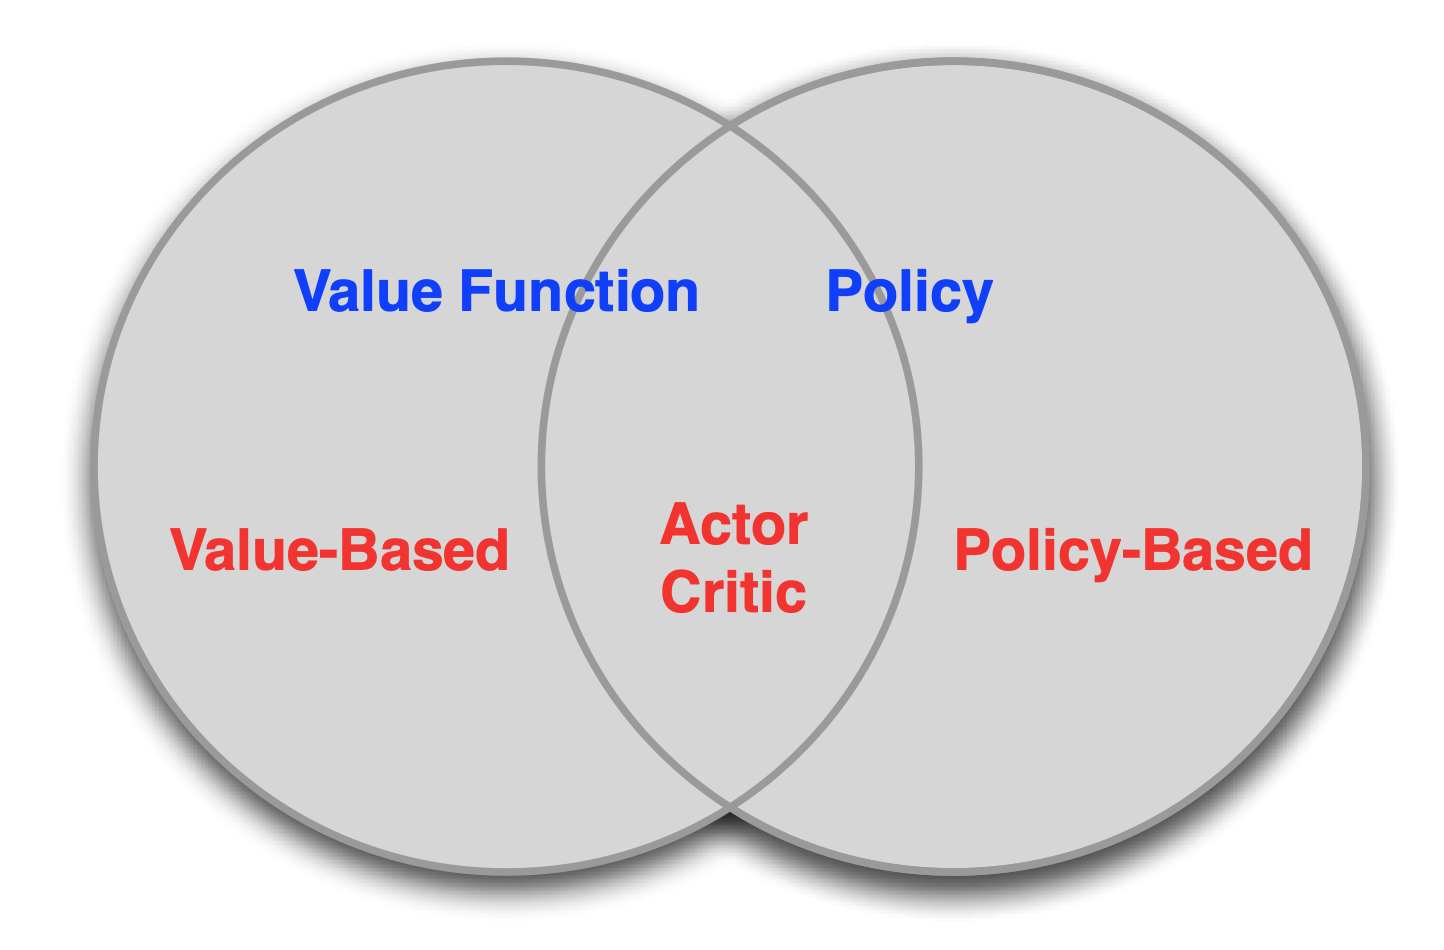
\includegraphics[width=0.75\linewidth]{rl_venn_diagram}
    \caption{Venn diagram relating the value-based algorithms like TD variants of $Q$-learning and SARSA, and policy-based algorithms like REINFORCE covered in this document. \footnotemark}
    \label{fig:basis_small_width}
    \end{center}
\end{figure}
\footnotetext{Source: \url{https://www.davidsilver.uk/wp-content/uploads/2020/03/pg.pdf}}

Actor-critic algorithms require us to a compute a state-value function, possibly in addition to an action-value $Q$-function, and certainly in addition to the policy function, which opens the question of how do we organize our algorithm to accomplish this goal? We can either learn the state-value function separately, or jointly in multi-task models with the action-value and/or policy functions. In fact, any splitting between the state-value, action-value, and policy functions is available to us, so that we may not have separate sets of parameters like $\boldsymbol{\theta}$ for the policy and $\boldsymbol{\phi}$ for the action- or state-value, but rather some parameters will be shared between them and other will not. 

Note that multi-task models are generally limited to neural networks and bespoke implementations. Moreover, they minimize a total loss \begin{equation}L_\text{total}=L_\text{actor}+L_\text{critic}+L_\text{regularizer}\end{equation} according to batch updates of Equation \ref{eq:simple_gradient_update}\cite{online_policy_gradient_review,openAI_part3}. For the critic, which predicts action- or state-values or both, the loss function depends on the difference between our predictions and the results returned from the environment, optionally bootstrapped off of prior predictions. For the normal distribution likelihood, we can use the squared error as in \begin{equation}\begin{split}L_\text{critic}^{\text{(state)}}&=\frac{1}{2}\mathop{\mathbb{E}}_{\boldsymbol{\tau}\sim\pi_{\boldsymbol{\theta}}}\left[\left(U_t-V(\mathbf{s}_{t})\right)^2\right]\\L_\text{critic}^{\text{(action)}}&=\frac{1}{2}\mathop{\mathbb{E}}_{\boldsymbol{\tau}\sim\pi_{\boldsymbol{\theta}}}\left[\left(U_t-Q(\mathbf{s}_{t},\mathbf{a}_t)\right)^2\right]\\L_\text{critic}^\text{(both)}&=L_\text{critic}^{\text{(state)}}+L_\text{critic}^{\text{(action)}}\end{split}\end{equation} Some variations may use the absolute error or the Huber loss. 

For the actor, i.e., the policy gradient, our loss function, according to Equations  \ref{eq:simple_gradient_update}, \ref{eq:policy_gradient_theorem}, and \ref{eq:policty_gradient_update}, is \begin{equation}L_\text{actor}=-\mathop{\mathbb{E}}_{\boldsymbol{\tau}\sim\pi_{\boldsymbol{\theta}}}\left[\sum_{t=0}^H\log\pi_{\boldsymbol{\theta}}(\mathbf{a}_t|\mathbf{s}_t)\Psi_t\right]\end{equation} Lastly, we can also add additional losses to our final optimized quantity, such as regularization losses to reduce the model complexity, or a self-entropy term \begin{equation}L_\text{regularizer}^\text{(entropy)}=\beta H(\pi, \mathbf{s})=-\beta \sum_a\pi(\mathbf{a}|\mathbf{s})\log\pi(\mathbf{a}|\mathbf{s})\end{equation} weighted (multiplied) by a chosen positive or negative hyperparameter $\beta$, to encourage more or less exploration as desired.  L1 and L2 regularizer losses are always available, written as \begin{equation}L_\text{regularizer}^{\text{(L2)}}=\beta\boldsymbol{\theta}^\top\boldsymbol{\theta}=\frac{\sigma^2}{\sigma_p^2}\boldsymbol{\theta}^\top\boldsymbol{\theta}\end{equation} where $\beta$ is the $L2$ regularization hyperparameter and $\sigma_p$ is a noise parameter scale hyperparameter which is equivalent to the average noise parameter for the prior, where the model parameters are all set to zero, or $\boldsymbol{\theta}=\mathbf{0}$. In addition, losses that allow us to simultaneously optimize either the homoskedastic the noise parameter $\sigma$, or the heteroskedastic noise parameter $\sigma(\mathbf{a},\mathbf{s})$, can be included, derived from the negative log of the normalization constant in a normal distribution, and which we can write as \begin{equation}L_\sigma=N_\text{data}\log\sigma\end{equation}such that $L_\text{regularizer}^\text{(L2)}$ and $L_\sigma$ balance each other out against the data fit term $L_\text{critic}$ and/or the policy gradient loss $L_\text{actor}$.

\section{Under the hood}

Stochastic gradient descent has the benefit of only ever needing to store and compute as many components as there are parameters in the model, as opposed to least squares methods that require storage of the square of the number of model parameters and computation of the cube. But the parameter update rules for the action- and state-value functions can be performed using any regression technique against the target $U_t$, including memory-based techniques. One such method, K-nearest neighbors regression, requires prediction order complexity $\mathcal{O}(k\times N_\text{data}\times N_\text{features})$ using brute force, or $\mathcal{O}(k\times \log(N_\text{data}))$ using a k-d tree or ball tree data structure. Another, Gaussian process regression (GPR), requires prediction order complexity $\mathcal{O}(N_\text{data}^3)$, which is much higher. Techniques for reducing the order complexity of the GPR revolve around selecting subsets of the training points, such as the Nystrom approximation\cite{nystrom}. 

For direct policy optimization, however, we are required to craft a custom loss function, which limits our techniques to methods with explicitly-defined loss functions. For example, almost all policy gradient implementations found online use neural networks, which come with infrastructure for defining a custom loss function and computing its gradient, but any algorithm that performs stochastic gradient descent over a custom loss function will also work. In special cases, the gradients can be analytically derived and programmed explicitly. 

For example, if we use a linear model for action preferences $h_{\boldsymbol{\theta}}(\mathbf{s},\mathbf{a})=\boldsymbol{\theta}^\top\mathbf{x}(\mathbf{s},\mathbf{a})$, where $\mathbf{x}(\mathbf{s},\mathbf{a})$ represents our observations or features covering both the state and the action, we can use the softmax function to define the policy as \begin{equation}\pi_{\boldsymbol{\theta}}(\mathbf{a}|\mathbf{s})=\frac{\exp[h_{\boldsymbol{\theta}}(\mathbf{s},\mathbf{a})]}{\sum_{\mathbf{a}'\sim\mathcal{A}}\exp[h_{\boldsymbol{\theta}}(\mathbf{s},\mathbf{a}')]}=\frac{\exp[\boldsymbol{\theta}^\top\mathbf{x}(\mathbf{s},\mathbf{a})]}{\sum_{\mathbf{a}'\sim\mathcal{A}}\exp[\boldsymbol{\theta}^\top\mathbf{x}(\mathbf{s},\mathbf{a}')]}\end{equation}We see that the gradients have an analytical form we can exploit to cheaply update the policy, given by \begin{equation}\frac{\partial \pi_{\boldsymbol{\theta}}(\mathbf{a}|\mathbf{s})}{\partial \boldsymbol{\theta}}=\pi_{\boldsymbol{\theta}}(\mathbf{a}|\mathbf{s})\mathbf{x}(\mathbf{s},\mathbf{a})\left(1-\frac{1}{\sum_{\mathbf{a}'\sim\mathcal{A}}\exp[\boldsymbol{\theta}^\top\mathbf{x}(\mathbf{s},\mathbf{a}')]}\right)\end{equation}
However, for more complex loss functions, it may be difficult to analytically define their derivatives, or we may prefer to automate the process to accommodate a wide range of loss functions we can't anticipate. In this case, a stand-alone automatic differentiator (like Python's \textit{autograd}) can be used, which works with regular functions that use a special imported version of \textit{NumPy} to help it keep track of the operations, although it can only handle certain operations and patterns that the user must be aware of. Unfortunately, problems that require any degree of simulation, or are undifferentiable, are not well suited to automatic differentiation.

While it would be possible to employ function optimization methods like SciPy 's minimize package to optimize either policy evaluators or the policy itself, or to use any other non-gradient based function optimizer, these will drive the loss to its optimum over a fixed dataset and this can produce poor results. This is because, unlike in supervised learning, we do not have a fixed distribution of data, but rather the data distribution changes as the parameters change. We can see that this is the case since our actor and critic losses and their gradients are defined as expectations over trajectories produced by the policies we are optimizing, rather than sums over all possibilities. In fact, it is because we measure our policies through the data distribution that they return to us that we can slowly learn optimal policies without any reinforcement learning tricks at all. 

This is a major achievement of both semi-gradient and policy gradient methods, since it brings us back to earth by allowing us to sample these expectations using the most recent policy, and with importance sampling, we can account for the data distribution drift in off-policy training. However, we must still keep in mind that the loss functions we compute at any step of optimization are limited by the expectations over trajectories we had to compute using a different policy than the one we end up with because it didn't exist yet. In other words, our goal is not to optimize the loss at any given stage of training, but to optimize the rewards of the system, which the losses help us achieve at each step. For these reasons, you will sometimes see an abuse of notation when the gradient update for policy evaluators is written as \begin{equation}\boldsymbol{\phi}=\argmin_{\boldsymbol{\phi}}\mathop{\mathbb{E}}_{\boldsymbol{\tau}\sim\pi_{\boldsymbol{\phi}}}\left[\left(U_t-Q(\mathbf{s}_t,\mathbf{a}_t)\right)^2\right]\end{equation} and similarly for policy gradients \begin{equation}\boldsymbol{\theta}=\argmin_{\boldsymbol{\phi}}\mathop{\mathbb{E}}_{\boldsymbol{\tau}\sim\pi_{\boldsymbol{\theta}}}\left[\log\pi_{\boldsymbol{\theta}}(\mathbf{a}_t,\mathbf{s}_t)\Psi_t\right]\end{equation}but it is important to remember that this is only true when we keep updating the distribution used to evaluate the expectation.

As a result, one rarely sees solutions that don't use gradient descent or require the tuning of a learning rate $\alpha$ hyperparameter. For exact, online methods, like Bayesian linear regression, we account for the changing data distribution of the loss function because each step of training amounts to adding new rows of data, so that we are ultimately minimizing or maximizing the average of the expectations over the history of the parameters, similar to stochastic gradient descent. It is up to numerical experiments to fine-tune $\alpha$, or the decay factor we use to drop out old rows of data, to see how the different methods compare. When using neural networks with gradient descent, it is also important to scale the inputs to the standard normal where the model has the most capacity, and to be aware that the model interpolates linearly through gaps of data, and extrapolates linearly outside the domain of the standard normal. This can be addressed by either stalling training until a data sample has been made, or one can apply batch normalization\cite{batch_normalization} as a regularization technique.

From an engineering perspective, note that the formalism for training the state- and value-functions, regardless of the target $U_t$, is equivalent to the formalism for \textit{contextual multi-armed bandits} (CMABs), and both align between versions with discrete and continuous actions. While both policy evaluator learning and bandits may train against targets compiled during a loop at the end of each episode that rewinds the previous actions, states, and rewards, only $Q$-learning incorporates the $\argmax_\mathbf{a}$ over future steps before it is reflected in the policy being trained thanks to the Bellman equation. This allows information about successful policies to propagate back to earlier steps before they are reflected in the policy used to collect data, making training in situations where planning is relevant much faster. Since we incorporate the unique qualities of $Q$-learning entirely during the collection loop that passes targets to the function approximator, we can use a CMAB under the hood for both training and prediction in the collection loop.  Direct policy optimization, meanwhile, enjoys a similar structure, except with a different loss function that doesn't strictly fit the regression structure.

Just as properties of the update algorithm made true gradient methods using the state- or action-value functions unstable, requiring the development of semi-gradient methods, certain combinations of algorithm properties can produce other instabilities. One particular combination, known as the \textit{deadly triad}, must be particularly avoided:
\begin{enumerate}
\item Bootstrapping the target $U_t$, i.e., using any target besides Monte Carlo such as TD
\item Off-policy training
\item Non-linear function approximation
\end{enumerate}
To learn more, see Section 11.3 in \cite{sutton_barto_rl}.

Using function approximation for both the policy evaluation and the policy itself necessarily implies partial observability of our environment, and while losing observations can kill our ability to learn a successful policy, the methods described here will do as well as we possibly can given the handicap. However, we can go the other way and add observations, too, and an obvious choice is to add historical data from earlier the trajectory. This can be accommodated by either encoding them as truncated and padded concatenations to the original feature vector, or by using sequential models like RNNs and LSTMs to encode the historical data into a fluid representation. In addition, there are a host of feature extraction, kernel approximation, convolution, and dimensionality reduction methods that can be employed, in parallel, serial, or along any directed acyclic graph (DAG) that defines your feature pipeline, as shown in Figure \ref{fig:ml_map}. But remember, as we add more expressiveness and/or features to our models, that is, as we add more parameters, we increase our model capacity but also dramatically reduce the speed at which it learns. A general rule of thumb is that by using $M$ times more features, it takes $M^2$ more samples to move out of exploration into exploitation.
\begin{figure}
\label{fig:ml_map}
    \begin{center}
    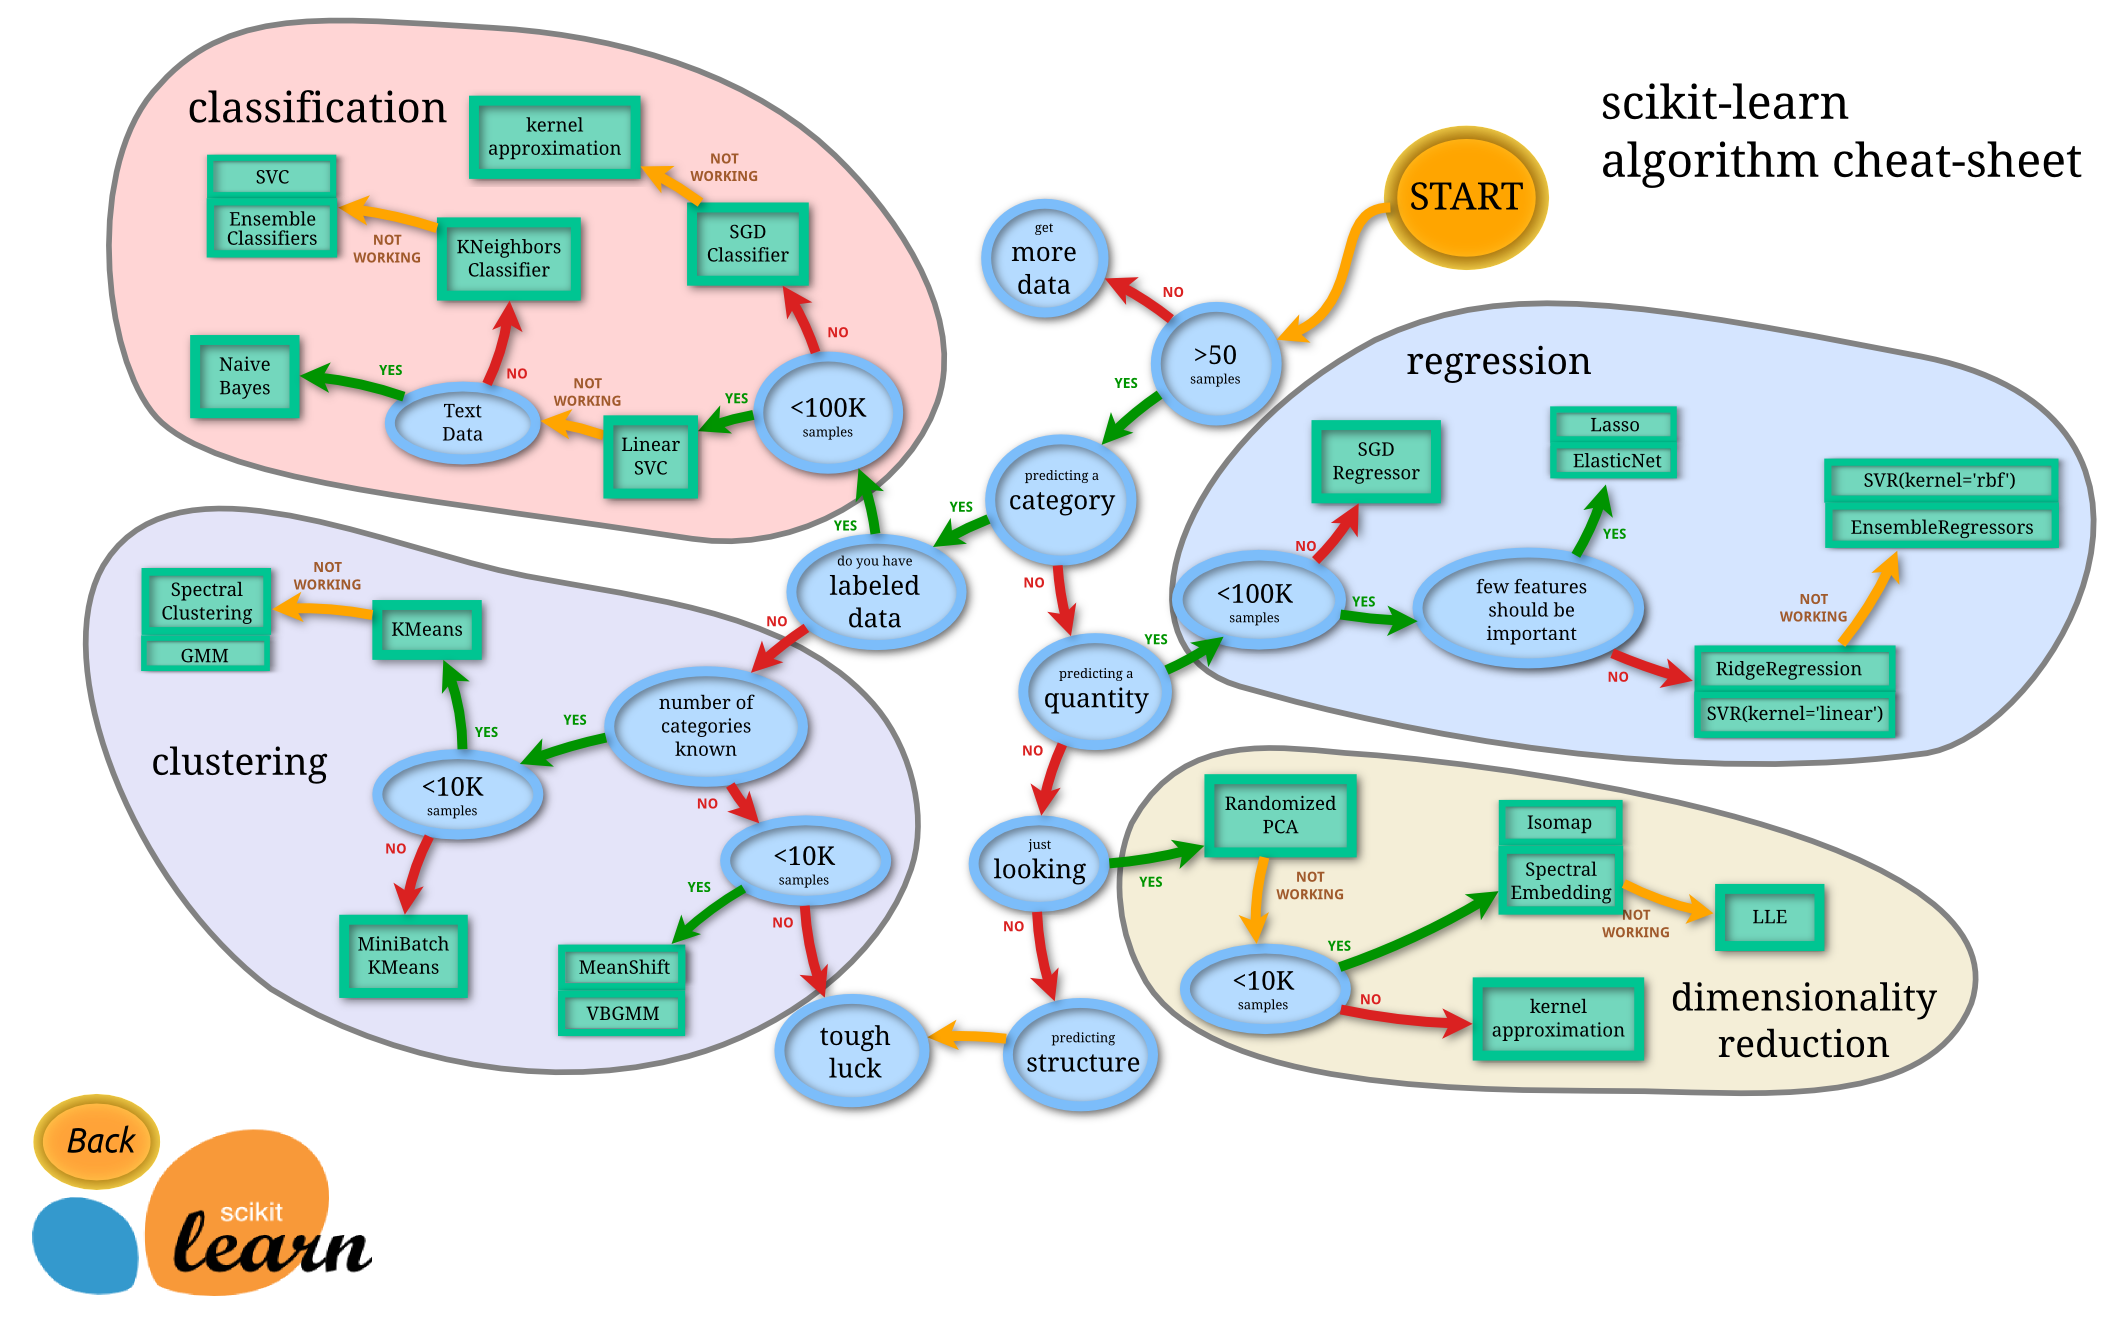
\includegraphics[width=0.75\linewidth]{ml_map.png}
    \caption{Building a feature extraction and transformation pipeline can be a challenge, and this flowchart is a terrific way to explore your options. The online version provides links to implementations in the Python package \textit{scikit-learn} \footnotemark}
    \end{center}
\end{figure}
\footnotetext{Source: \url{https://scikit-learn.org/stable/tutorial/machine_learning_map/index.html}}

Moreover, policy and action-value functions generally only work when we incorporate interaction features between the state and action features, except for decision-tree based algorithms like random forests and gradient-boosted trees, whereas neural networks are designed to learn which interactions are most useful at the cost of extensive hyperparameter tuning. Since there are so many ways to add features, we can bring down the complexity of these computations and to help our agents learn faster by applying randomized projections onto any subset of our feature space, but this also introduces additional hyperparameters to tune. We recommend randomized projections over Principle Component Analysis (PCA) since random projections to not require an input data sample before we can train our function approximators, and because there is no particular reason to expect the signal to be insensitive to the low-variance features that are filtered out in PCA. Other options for dimensionality reduction include manifold learning, which also require data sampling, and for which there are many options, including VAE, t-SNE, and spectral embedding. See \url{https://scikit-learn.org/stable/modules/manifold.html#spectral-embedding} for a list of well-implemented options.

Interestingly, there is a parallel for randomized projections in the kernel space, for problems that are better served that way. As covered in \cite{GP_BLR}, we can project our inputs into basis functions that allow us to use a linear regression to approximate an equivalent Gaussian. This allows us to perform regressions in the feature space, for example, by using Bayesian linear regression, with order complexity $\mathcal{O}(N_\text{basis})$ for gradient methods and  $\mathcal{O}(N_\text{basis}^3)$ for exact methods, as opposed to Gaussian process regression with order complexity $\mathcal{O}(N_\text{data}^3)$, all while approximating the kernel regression. Popular choices here include the Nystrom and Random Fourier Features.

When computing the $\argmax_\mathbf{a}$ for $Q$-learning style algorithms, we may run into difficulties for problem spaces with continuous or large action spaces. However, we have several options at play. The first is to simply sample the action space randomly and rank the predicted $Q$-values for all of them. This is a popular approach in derivative-free Bayesian optimization. If the action space is continuous, another option is to apply gradient ascent, but this can be computationally expensive. And lastly, we can encourage exploration by using Thompson sampling when sampling for the $\argmax$, as in \cite{RLSVI}.

\section{Additional resources}
Additional resources can be found below:
\begin{itemize}
\item RLlib from Ray covers different algorithms and whether they can accept discrete or continuous actions, as well as additional support such as sequential models, multi-agent implementations, and multi-GPU training. See \url{https://docs.ray.io/en/latest/rllib-algorithms.html}
\item Lilian Wang has created one of the most thorough overview of policy gradient based algorithms at \url{https://lilianweng.github.io/lil-log/2018/04/08/policy-gradient-algorithms.html}
\item Spinning Up from OpenAI offers a terrific overview of reinforcement learning concepts as well as deep dives (and implementations) of some of the more advanced algorithms such as Proximal Policy Optimization (PPO), Deep Deterministic Policy Gradient (DDPG), and Soft Actor-Critic (SAC). However, some of their explanations, such as around the policy gradient, can be obscure and needlessly confusing. See \url{https://spinningup.openai.com/en/latest/}
\item David Silver's lecture slides at University College London are a legendary resource for succinct coverage of the main concepts in reinforcement learning. See \url{https://www.davidsilver.uk/teaching/}
\item Julien Vitay provides a sprawling overview of deep reinforcement learning at \url{https://julien-vitay.net/deeprl/Introduction.html}
\end{itemize}

\printbibliography
\end{document}
